% !TEX root =  paper.tex

\section{Evaluation}
\label{section:evaluation}

To evaluate \toolname, we conducted 
qualitative and quantitative studies 
aiming at answering the following research questions:

\begin{enumerate}[label=\textbf{RQ\arabic*},leftmargin=*]

	\item Are the refactorings by \toolname's component generation correct?

	\item How effective is \toolname 
	in identifying UI components compared to manual examination by web developers?
	
	\item How much code reusability can be achieved through the proposed refactorings? 
	
\end{enumerate}

In the following subsections, we discuss the details of the experiments
that we designed to answer each research question,
together with the results.

\subsection{RQ1: Correctness of Component Generation Refactorings}

\subsubsection{Study Design}

For the proposed componentization applied on \html to be safe, 
the main criterion is that the original and the refactored {\html}s 
must result into the same \dom tree landed into the users' web browsers.
Consequently, to devise a technique that can automatically assess 
the safety of the applied transformations,
we relied on the equivalence of the \dom subtrees 
rendered in the web browser,
before and after refactoring.
If the \dom trees are the same, given that our refactorings do not change
any \css style rules, the resulting presentation semantics of the \html files remain intact. 

To automate this process, we serialized the final \dom trees rendered in the browser
to the pretty-printed \html code and compared them pre- and post-refactoring.
This allows a fast comparison of the structure of the \dom trees.
We normalized the \dom trees by removing text nodes which are empty or contain only white spaces.
This is done because \react interprets these nodes differently~\cite{React:WhitespaceIssue, React:JSXWhiteSpaces} compared to the standard \html specifications.

\subsubsection{Results and Discussion}
Using the aforementioned technique, 
we compared the \dom subtrees of the UI component instances
before and after refactoring for the \totalNumberOfComponentInstances UI component instances 
(i.e., \numberOfComponents UI components) identified by \toolname.
The tests has passed for all subjects,
indicating that the refactorings introduced by component generation do 
preserve the \dom trees,
and as a result, the transformations are safe to apply.


\subsection{RQ2: UI Component Identification}

\subsubsection{Study Design} 
\label{sec:study-design}

We asked independent expert web developers to participate in a qualitative study,
with the goal of understanding what they would identify as
being a component pattern in a web UI. 
With this study, we aim at evaluating the (dis)agreement between the proposed approach and expert developers in terms of identifying the UI components.



\header{Subject Systems}
We searched the Internet to find mockups suitable for this study
(using keywords like ``web mockups'', ``web templates'', ``front-end templates'').
Our selection criteria for choosing mockups were:

\begin{itemize}[leftmargin=*]
	\item They should be non-trivial, both visually 
	and code-wise (i.e., \html and \css).
	Note in \Cref{table:mockup-complexity} that
	the mockups are indeed complex,
	in terms of the number of \dom nodes and \css code size.
		
\item The number of subjects should be small and manageable enough	
	so that we can ask participants to highlight potential components 
	in \emph{all} of them,
	without causing too much burden, mental fatigue, or boredom on them
	which can negatively distort the study.

	\item They should only represent the UI front-end,
	i.e., without back-end or front-end business logic or functionalities.
\end{itemize}

Based on these criteria we chose \numberOfTemplates mockups for our evaluation. We use the same mockups in all the evaluation experiments.
\Cref{table:mockup-complexity} shows descriptive statistics
for them.

\begin{table}
	\caption{Subjects' descriptive statics}
	\centering
	%\fontsize{8pt}{9.2pt}\selectfont
	%\setlength\tabcolsep{2px}
	\begin{threeparttable}
		\bgroup
		%\def\arraystretch{1.2}
		\begin{tabular}{c r r r}
			\toprule
			\textbf{Subject\#} & \textbf{Body size (KB)} & \textbf{\#\dom nodes} & \textbf{\css size (KB)\tnote\textdagger} \\ \toprule
			        1          & 18                       & 754                   & 323                                      \\
			        2          & 20                       & 915                   & 279                                      \\
			        3          & 33                       & 1,990                 & 350                                      \\
			        4          & 24                       & 1,226                 & 330                                      \\
			        5          & 49                       & 1,065                 & 254                                      \\ \bottomrule
		\end{tabular}
		\egroup
		\begin{tablenotes}
			\item[\textdagger] Some mockups use \css frameworks (e.g., Bootstrap).
			This corresponds to the total \css size, including the frameworks.
		\end{tablenotes}
	\end{threeparttable}
	\label{table:mockup-complexity}
\end{table}



\header{Participants} 
We emailed developers who have worked in local businesses or research labs
and asked them to voluntarily participate in our study.
We attached a zip package containing our subject systems 
together with a link to a post-study questionnaire aimed at collecting information about the participants' demographics
(e.g., number of years of experience in software engineering in general and in web development in particular,
and their self-assessment on web application development skills).
We asked them to manually highlight repetitions on the UI of each subject (by drawing a rectangle on each repetition) and send the results back to us.

Accordingly, we emailed 10 developers and informed them of the study, and asked them to also pass it on to their contacts. We received responses from a total of \numberOfParticipants developers.
\Cref{table:participants-demographics} shows participants'  demographic information.
As it is shown, all the participants were quite experienced in web development,
as measured by the years of software and web development experience
and their own self assessment.

\begin{table}[b]
	\caption{Demographics of the Participants}
	\centering
	%\fontsize{8pt}{9.2pt}\selectfont
	%\setlength\tabcolsep{2px}
	\begin{threeparttable}
		\bgroup
		%\def\arraystretch{1.2}
		\begin{tabular}{c c c c}
			\toprule
			\multirow{2}{*}{\textbf{Participant\#}} & \textbf{SW dev.}   & \textbf{Web dev.}  & \textbf{Web dev. self assessment} \\
			                                        & \textbf{(\#Years)} & \textbf{(\#Years)} & \textbf{(1--5, 5=Highly Expert)}  \\ \toprule
			                   1                    & 10                 & 5                  & 4                                 \\
			                   2                    & 8                  & 2                  & 4                                 \\
			                   3                    & 3                  & 3                  & 4                                 \\
			                   4                    & 11                 & 3                  & 3                                 \\
			                   5                    & 9                  & 8                  & 5                                 \\ \bottomrule
		\end{tabular}
		\egroup
	\end{threeparttable}
	\label{table:participants-demographics}
\end{table}

\header{Comparison with Developers}
For each subject, we compared the components highlighted by the experts 
with those components that \toolname automatically identified as UI components.
In particular, when more than half of the experts
highlighted a pattern on the mockup as repeated, 
we assume the majority is correct and consider it as a UI component  
that our technique should be able to identify.
The performance of \toolname is then determined using the well-known \textit{precision} and \textit{recall} measures.
A \textit{true positive} for the approach is defined as a UI component that has been manually identified
by more than half of the experts (in our case, three or more participants).
A \textit{false positive}, on the other hand, is a UI component that is reported 
by the approach, yet less than half of the experts have identified it.
Finally, a \textit{false negative} of the approach
is a UI component that is reported by more than half of the experts, 
but the approach could not identify.

\subsubsection{Results and Discussion}
\Cref{table:comparison-results} shows the results of comparing the UI patterns identified by our approach to the UI patterns identified by participating developers in our experiment.
The table shows the values for true positives, false positives, false negatives, and finally precision and recall. 
The values for recall range between 74\% and 100\%. We examined the subjects at the lower end of the range to investigate further.
Almost all the components that were missed by our approach had many elements that had animations or moving sub-elements (e.g., a carousel that changes every few seconds). 
Our technique was not designed with animations in mind.
Capturing and analyzing animations can be challenging, due to difficulties in keeping track of changes over time and deciding which time instant to take as representative. This might be a possible venue for future work.


%\begin{table*}
\begin{sidewaystable}
	\centering
	\caption{Comparison of automatically identified components to manually-identified ones by developers}
	\label{table:comparison-results}
	%\setlength\tabcolsep{3px}
	\begin{threeparttable}
		\begin{tabular}{c c c c c c r r | c r r}
		\toprule
		\multirow{2}{*}{\textbf{Subject}}
						& \multicolumn{2}{c}{\textbf{\#Identified Refactoring Opportunities}}
														& \multirow{2}{*}{\textbf{FN}}
																& \multirow{2}{*}{\textbf{TP}} 
																		& \multirow{2}{*}{\textbf{FP}}
																				& \multirow{2}{*}{\textbf{Precision}}
										 													& \multirow{2}{*}{\textbf{Recall}} 
										 																& \multicolumn{3}{c}{\textbf{Considering PMO}\tnote{\textdagger}}
														 												\\ \hhline{~--~~~~~---}
						& \textbf{\scriptsize \#Components}
										& \textbf{\scriptsize \#Component Instances}
														& 		&		& 		&  			&			&  \textbf{{\#}PMO}		& \textbf{Precision} 
																															& \textbf{Recall} 	\\ \toprule
		1 				& 5				& 29			& 0 	& 19	& 9 	& 67.9\% 	&  100.0\% 	& 8	& 96.4\%	& 77.1\%            \\
		2 				& 5				& 27			& 0 	& 15	& 2  	& 88.2\%  	&  100.0\%  & 2	& 100.0\%	& 77.3\%			\\
		3 				& 5				& 26			& 6 	& 17	& 5 	& 77.3\%  	&  73.9\%   & 0	& 77.3\%	& 68.0\%			\\
		4 				& 6				& 21			& 3 	& 9		& 12 	& 42.9\%   	&  75.0\%   & 12	& 100.0\%	& 84.0\%			\\
		5 				& 4				& 17			& 3 	& 13	& 4 	& 76.5\%   	&  81.3\%   & 3	& 94.1\%	& 69.6\% 			\\ \midrule
		\textbf{Avg.}	& \textbf{5}	& \textbf{22}	&		& 		&   	& \textbf{70.5\%}	
																							& \textbf{86.0\%}  	
																										& \textbf{5} 
																												& \textbf{93.6}\%  		
																															& \textbf{75.2}\% \\ \bottomrule
		\end{tabular}
		\begin{tablenotes}
			\item[\textdagger] PMO = Potentially Missed Opportunities.
		\end{tablenotes}
	\end{threeparttable}
%\end{table*}
\end{sidewaystable}

As for the precision, we further examined the nature of false positives in order to better understand the performance.
Following this examination, we identified another variable while performing the comparison with participants: the \emph{potentially missed opportunities}.
We define missed opportunities as those patterns that were reported by as few as one developer (but not the majority), \emph{as well as} our tool.
The reason for introducing this variable is that, by manually examining the false positives,
we noticed that there were a few potential opportunities that were missed by the majority of developers.
We postulate a number of possible causes as to why such patterns were not reported by the majority of participants:

\begin{itemize}[leftmargin=*]
\item Some repeating components were laid out far away from each other (e.g., at the very top and very bottom of the page).
This often makes it difficult for human developers to remember patterns that are not immediately visible within the same view, especially if there are lots of patterns that they have to keep track of.
The human brain has been shown to have a short-term memory capacity of only around 3 to 7 objects at a time \cite{memory_limit_cowan_2001}. This fact, coupled with patterns that are far away from each other and interlaced with multiple other patterns, can cause humans to miss some patterns.
Our approach, however, is agnostic to where the pattern is located, and is able to recognize matching patterns from far ends of a web UI just as easily as patterns immediately next to each other.

\item Some components included images or icons that were designed to be faint or barely visible due to artistic reasons.
Such icons, especially when present close to very vibrant and large repeating components,
are often skipped potentially due to the visual attention in the brain being directed at the larger clearer patterns.
However, due to the visual normalization adopted in our approach, such artistic choice do not make any difference and the pattern is recognizable regardless of how visually pronounced it is.

\end{itemize}


\subsection{RQ3: Code Reusability}

\subsubsection{Study Design}

We now proceed to determine how much code reusability can be attained with the components generated by the approach. For each test subject, we compare the size of the \html code of the mockups before and after refactoring as a measure of how much reusability has been achieved.

Let $T_r$ be the set of \dom subtrees corresponding to the UI component instances
which are going to be removed by a refactoring operation, $r$, from the original \html.
The refactoring $r$ adds the necessary code
which unifies $T_r$ subtrees into a UI component $u_r$
to the original \html code.
Moreover, $r$ replaces $T_r$ subtrees with a set $C_r$ of calls to instantiate $u_r$.
Accordingly, the size reduction $SR_r$ for the refactoring $r$ is computed as:
\begin{equation}
SR_r = \sum\limits_{t \in T_r}{sizeOf(t)} - sizeOf(u_r) + \sum\limits_{c \in C_r}{sizeOf(c)}
\end{equation}

\noindent 
where $t$ is a component instance, $c$ is a component instantiation call, and $sizeOf(x)$ is the number of bytes corresponding to $x$
when serialized to \html. 
In an \html mockup, there might be several 
sets of component instances
(i.e., several UI components might be created).
The overall size reduction $SR$, which is achieved by applying 
the set $R$ of all refactoring opportunities
found in a mockup, is calculated as {\footnotesize$SR = \sum\limits_{r \in R}{SR_r}$}.

We calculate the size reduction in two different ways:
1) based on an implementation using a UI framework (which we have chosen to be \react),
and 
2) based on the representation contained in the \model.
This is because each UI framework (e.g., \react, \angular) has its own syntax and idiomatic mechanisms 
for creating UI components and instantiating them.
As a result, the actual size reduction would be different depending on which, and how, a UI framework is used.
All UI frameworks, however, follow the same basic principle:
the set of \dom nodes that can be unified into single \dom nodes
form a \textit{template} for the UI component, 
while other nodes form the \textit{parameters} (i.e., \textit{placeholders}) in the UI component.
These placeholders are filled with the \textit{arguments} passed when calling the UI framework.
As a result, calculating the size reduction based on the nodes
and arguments identified when constructing the \model
allows a more accurate determination of how the algorithm \emph{intrinsically} performs
in terms of code reusability,
regardless of the differences between the many possible UI frameworks that can be used.

Moreover, when using a third-party UI framework,
it is usually required that the framework's \javascript library code is imported at the client-side
so that the web browser is able to render the UI,
potentially increasing the overall size of the client-side code.
However, if the web application wants to enjoy
the maintainability benefits of the UI framework,
the \javascript files should be imported anyway.
As mentioned, this is an extensively-popular trend 
among the developers~\cite{StateOfJS:WebPlatformTests, StackOverflow:2017:Survey}.
Notwithstanding, if developers opt for using standard \html Web Components ~\cite{MDN:2017:WebComponents}
instead of third-party UI frameworks,
there will be no burden in terms of the additional imported \javascript files.
As a result, when reporting the size measurements for \react,
we only consider the code generated by our approach for implementing UI components,
not \react's own core \javascript code.


\subsubsection{Results and Discussion}

\begin{figure}
    \centering
    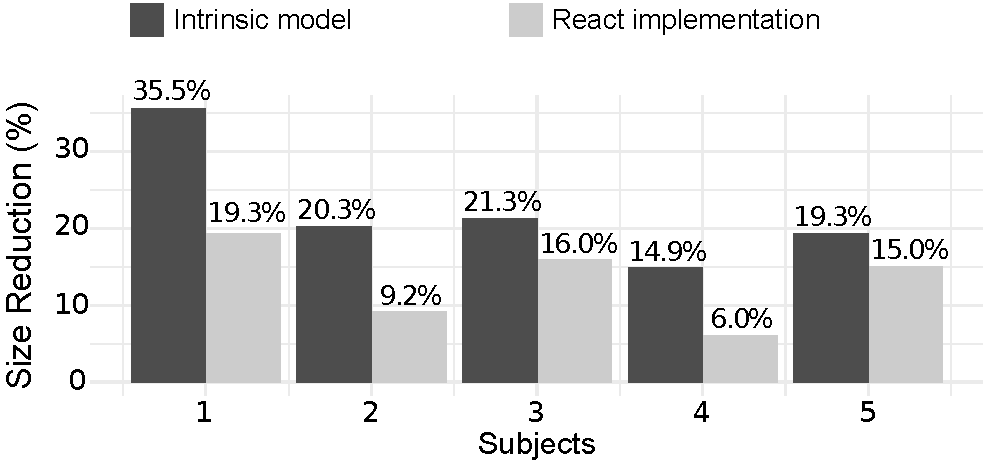
\includegraphics[width=0.75\textwidth]{maintainability/figures/size-reduction}
    \caption{Code reusability achieved by the proposed component generation, as measured by final size reduction.}
    
    \label{fig:size-reduction-results}
\end{figure} 

\begin{comment}

\begin{table}
	\caption{Size Reduction in the Mockup's \html}
	\centering
	%\fontsize{7pt}{8pt}\selectfont
	\setlength\tabcolsep{3px}
	\begin{threeparttable}
		%\bgroup
		%\def\arraystretch{1.4}
		\begin{tabular}{c c c c r r}
			\toprule
			\multirow{2}{*}{\textbf{Subject}}
				& \multicolumn{2}{c}{\textbf{\#Identified Refactoring Opportunities}} 
								&	& \multicolumn{2}{c}{\textbf{\%Size Reduction}}  \\ 
				\hhline{~--~--}
				& \textbf{\#Components}
						& \textbf{\#Component Instances}
								& 	& \textbf{Algorithm}
											& \textbf{\react} \\  \toprule
			1	&  5	& 29	&	& 35.54	& 19.34 \\
			2	&  5	& 17	&	& 20.27	&  9.20 \\
			3	&  5	& 26	&	& 21.33	& 16.00 \\
			4	&  6	& 21	&	& 14.90	&  6.01 \\
			5	&  4	& 17	&	& 19.34	& 15.01 \\ \midrule
\textbf{Avg.}	&  \textbf{5}	
						& \textbf{22}	
								&	& \textbf{18.96}
										 	& \textbf{11.56}  \\ \bottomrule
		\end{tabular}
		%\egroup
	\end{threeparttable}
	\label{table:size-reduction-results}
\end{table}

\end{comment}


\Cref{fig:size-reduction-results} illustrates the results of applying the proposed refactorings
on the test subjects.
Observe that, using \react implementation,
refactoring UI components results in reducing the size of the \html code
by 6\%--19.34\%, with an average of 11.56\%.
The \textit{intrinsic} performance of the algorithm itself, however, is higher: 14.90\%--35.54\%,
with an average of 18.96\%.
This difference highlights that \react components require quite considerable amount of added code
to the original \dom information of the UI component instances.
For example, a UI component shown in \Cref{fig:intermediate-model-sample-dom-subtrees}(d)
needs to be wrapped into a function named \code{render} implemented in a
\javascript class that extends the internal \react class, \code{React.Component}.
We also need to add additional code to pass arguments to the UI components for each UI component instance.
As mentioned, using another UI framework can yield different saving ratios. It is for these reasons that reporting the intrinsic performance is important.

It is worth mentioning that this saving is not meant to replace existing techniques
that, for instance, minify \html by removing white space, or via any other reduction approach.
Rather, whatever savings obtained from the components can complement them by adding even more saved bytes on top of what they would normally save.


\section{Discussion}
\header{Context within web development} The approach we present in this chapter refactors repetitions in the UI and merges them into a template, which is finally converted into a component in one of the common front-end frameworks (e.g., \react, \angular). This automates one of the initial steps in making a full-fledged web app UI, which is often time consuming and is done manually. The use of this approach, of course, would not mean that the web app is ready to launch to clients and the development process is finished. The developer would use these components and continue the development, by, e.g., adding business logic, handling events, connecting to databases or other sources. Furthermore, the approach we present in this chapter is for modularizing the UI view itself, and is therefore orthogonal to the remaining components of the architecture pattern of the app (e.g., Model-view-controller (MVC), Model-view-presenter (MVP)) and to any backend server functionality.

\header{Threats to validity}
We chose test subjects (i.e., mockups) randomly from the Internet
with the mentioned criteria in \Cref{sec:study-design},
to avoid any selection bias.
Plus, the evaluation participants are expert web developers
with different years of web development experience,
mitigating the threats to the internal validity of the study.
The mockups are diverse and complex enough
to be representative of real-world app front-ends,
mitigating the external validity of the study by making the results generalizable.
To make the study replicable, we have made 
\toolname's source code, evaluation subjects, and the anonymized participants' responses available online~\cite{tool-and-data}.